
\documentclass[11pt, aspectratio=169]{beamer}

\usepackage[utf8]{inputenc}
\usepackage{tikz}
\usepackage[english]{babel}
\usepackage{svg}
\usepackage{eurosym}
\usepackage{subfig}
\usepackage{pgfgantt}
\usepackage[export]{adjustbox}
%\usepackage[shortlabels]{enumitem}
\usepackage[font=scriptsize,justification=centering]{caption}
\usepackage{movie15}
\graphicspath{{figures/}}

%----------------------------------------------------------------------------------------
%   TITLE PAGE INFORMATION.
%----------------------------------------------------------------------------------------
\author{S. Björk, J. Hooper, J. M. Inga, H. Magnusson, A. Śmiałek}
\title{InfraRed Imaging of astronomical targets with a Stabilised Camera}
\subtitle{IRISC}
\institute{ESA ESTEC, Noordwijk}
\date{13-17 April 2019}
%\subject{} 

%----------------------------------------------------------------------------------------
%   SETUP LAYOUT.
%----------------------------------------------------------------------------------------
\usepackage{theme/beamerthemeWarsawLTU}
%\usetheme{Warsaw}


\begin{document}
%----------------------------------------------------------------------------------------
%   TITLE PAGE.
%----------------------------------------------------------------------------------------

{\setbeamertemplate{logo}{}
\begin{frame}
\titlepage
\begin{tikzpicture}[remember picture,overlay]
    \node[xshift=13cm,yshift=-1.025\textheight,anchor=north west] at (current page.north west){%
    \includegraphics[width=2cm]{theme/LTU_logo.jpg}};
\end{tikzpicture}
\end{frame}
}

%----------------------------------------------------------------------------------------
%   TABLE OF CONTENTS.
%----------------------------------------------------------------------------------------
\begin{frame}[t]{Table of Contents}
\vspace{-0.3cm}
    \begin{columns}[t]
        \begin{column}{.5\textwidth}
            \tableofcontents[sections={1-2}]
        \end{column}
        \begin{column}{.5\textwidth}
            \tableofcontents[sections={3-5}]
            \vspace{-.2cm}
            \tableofcontents[sections=6,hidesubsections]
        \end{column}
    \end{columns}
\end{frame}


%----------------------------------------------------------------------------------------
%   INTRODUCTION.
%----------------------------------------------------------------------------------------

%----------------------------------------------------------------------------------------
%   SCIENCE.
%----------------------------------------------------------------------------------------
\section{Science}

%----------------------------------------------------------------------------------------
%   SYSTEM.
%----------------------------------------------------------------------------------------
\section{System}
%   CONSTRUCTION. -----------------------------------------------------------------------
\subsection{Construction}
%   THERMAL. ----------------------------------------------------------------------------
\subsection{Thermal}
%   ELECTRICAL. -------------------------------------------------------------------------
\subsection{Electrical Setup}
%   SOFTWARE. ---------------------------------------------------------------------------
\subsection{On-board Software}

%%%%%%%%%%%%%%%%%%%%% states
    \begin{frame}[c]{Software - State Chart}
        \centering
        \begin{figure}
            \includegraphics[width=.7\textwidth]{software/state-diagram.png}
        \end{figure}
    \end{frame}
    %%% outer connections
            % power
            % datalink
%%%%%%%%%%%%%%%%%%%%% flow
    \begin{frame}[c]{Software - Activity}
        \centering
        \begin{columns}[t]
            \begin{column}{.5\textwidth}
                Low activity ``sleep'' during ascent\\
                \vspace{1cm}
                \only<2->{
                    Switch conditions:
                    \begin{itemize}
                        \item Current target leaves operational field of view
                        \item Target moves too close to the sun for observation
                        \item A higher priority target enters the field of view
                    \end{itemize}
                }
            \end{column}

            \begin{column}{.5\textwidth}
                \vspace{-1 cm}
                \begin{figure}
                    \includegraphics[height=.9\textheight]{software/activity-diagram.png}
                \end{figure}
            \end{column}
        \end{columns}
    \end{frame}

%%%%%%%%%%%%%%%%%%%%% uplink
    \begin{frame}[c]{Software - E-link Uplink}
        \centering
        \begin{columns}[t]
            \begin{column}{.5\textwidth}
                Basic commads:
                \begin{itemize}
                    \item Rebooting
                    \item Updating targets
                    \item Calibrating tracking
                    \item Controlling downlink
                    \item Setting camera settings
                    \item Guiding / Sanity
                    \item Cut Off
                \end{itemize}
            \end{column}

            \begin{column}{.5\textwidth}
                \only<2->{
                    \vspace{1cm}\\
                    \large{Maximum data rate:\\a few kbit/s}
                }
            \end{column}
        \end{columns}
    \end{frame}

%%%%%%%%%%%%%%%%%%%%% downlink
    \begin{frame}[c]{Software - E-link Downlink Load}
        \centering
        \begin{tabular}{| l | l | l | l |}
            \hline
            \textbf{Item} & \textbf{File size} & \textbf{Downlink rate} & \textbf{Datarate} \\\hline\hline

            NIR camera        & 20\,MB    & variable              & 440\,kbit/s  \\\hline
            Guiding camera    & 2\,MB     & 60\,s / on request    & 270\,kbit/s  \\\hline
            Sanity camera     & 4\,MB     & on request            & -            \\\hline
            Sensors           & 100\,B    & 1\,s                  & 1\,kbit/s    \\\hline
        \end{tabular}
    \end{frame}


%   GROUND STATION?. --------------------------------------------------------------------
\subsection{Ground Station}

    \begin{frame}[c]{Software - Ground Station}
        Role:
        \begin{itemize}
            \item Send telecommands
            \item Receive and display telemetry
        \end{itemize}
    \end{frame}

%   CONTROL. ----------------------------------------------------------------------------
\subsection{Control System}

\begin{frame}{Control system}
    Objectives of the control system:
    \begin{itemize}
        \item Selection and tracking the astronomical targets
        \item Stabilisation the telescope during exposure
        \item Avoid pointing the telescope at the Sun
        \item Thermal control of the CMOS sensor and the electronics box
    \end{itemize}
\end{frame}

\begin{frame}{Control system}
    \begin{itemize}
        \item<1-> Selection of targets: %\\
        \begin{itemize}
            \item Based on prioritisation parameters (e.\,g. brightness, location)
            \item Sensor data: star tracker, GPS %\\
        \end{itemize}
        \item<2-> Tracking of targets: 
        \begin{itemize}
            \item Model of movements of astronomical targets
            \item Sensor data: internal clock, GPS
        \end{itemize}
        \item<3-> Stabilisation of the gimbal: dynamic control system (e.\,g.~PID) %\\
        \begin{itemize}
            \item Mechanical model of the gimbal, motors model
            \item Sensor data: gyroscopes, encoders%\\
        \end{itemize}
        \item<4-> Feedback loop, measured states: 
        \begin{itemize}
            \item Kalman filter determines exact position \& orientation
        \end{itemize}
    \end{itemize}
\end{frame}

\begin{frame}[t]{Control system}
    \begin{figure}
        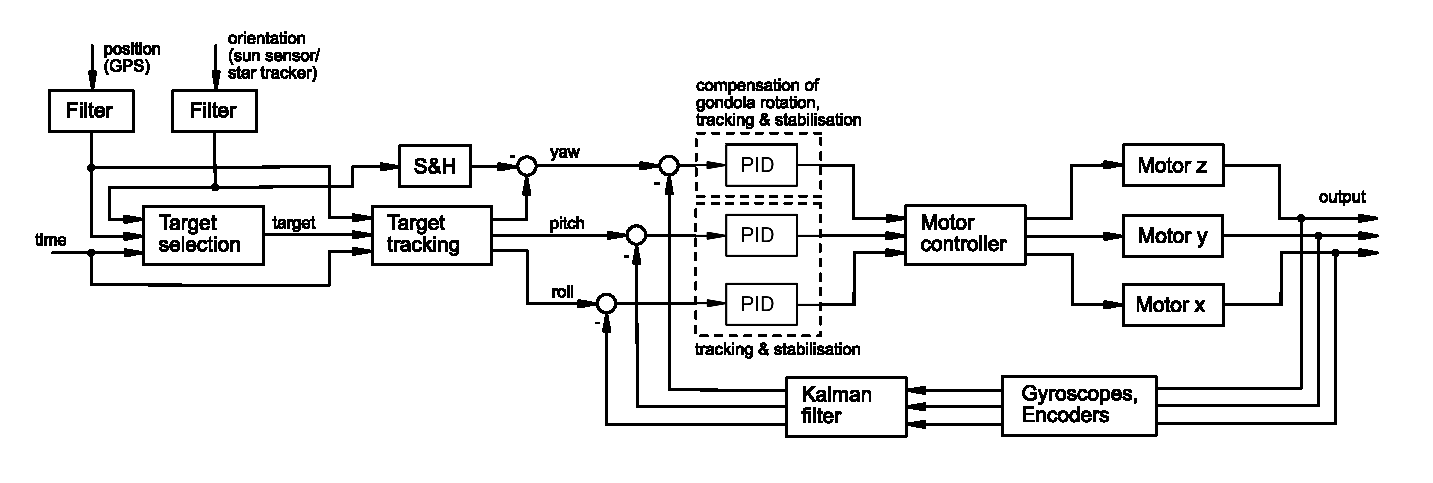
\includegraphics[width=\linewidth]{figures/images/Control_loop.eps}
        \caption{Main control loop}
    \end{figure}
\end{frame}
%   CAMERA. -----------------------------------------------------------------------------
\subsection{Cameras}
%   TELESCOPE. --------------------------------------------------------------------------
\subsection{Telescope}

%----------------------------------------------------------------------------------------
%   REQUIREMENTS AND RISKS.
%----------------------------------------------------------------------------------------
\section{Requirements and risks}
%   REQUIREMENTS. -----------------------------------------------------------------------
\subsection{Requirements}
%   RISKS. ------------------------------------------------------------------------------
\subsection{Risks}

%----------------------------------------------------------------------------------------
%   PROJECT MANAGEMENT.
%----------------------------------------------------------------------------------------
\section{Project Management}
%   TEAM. ---------------------------------------------------------------------------
\subsection{Team composition}
%   PLANNING. ---------------------------------------------------------------------------
\subsection{Time planning}
%   BUDGET. -----------------------------------------------------------------------------
\subsection{Budget}
%   OUTREACH. ---------------------------------------------------------------------------
\subsection{Outreach}

%----------------------------------------------------------------------------------------
%   SUMMARY.
%----------------------------------------------------------------------------------------
\section{Summary}

%----------------------------------------------------------------------------------------
%   QUESTIONS.
%----------------------------------------------------------------------------------------
\section{Questions}

%\begin{frame}[plain]{}
%%    \label{slide:questions}
%%    \centering
%%    \vspace{-0.71cm}
%%    \begin{figure}
%%    \hspace*{-1.1cm}
%%      \includegraphics[width=1.15\textwidth]{figures/images/teamphoto.png}
%%    \end{figure}
%   \includegraphics[width=\paperwidth]{figures/images/IRISC_Team_001_16_9+logo.jpg}
%\end{frame}
{
\usebackgroundtemplate{\includegraphics[width=\paperwidth]{figures/images/IRISC_Team_001_16_9+logo.jpg}}
\begin{frame}[plain]
\label{slide:questions}
\end{frame}

}
%----------------------------------------------------------------------------------------
%   BACKUP SLIDES.              EVERYONE!!!
%----------------------------------------------------------------------------------------

\begin{frame}[c]{Software Composition}
    \centering
    \includegraphics[height=.9\textheight]{software/composition-tree.png}
\end{frame}

\end{document}
